\documentclass[12pt,a4paper]{article}
\usepackage[polish]{babel}
\usepackage[T1]{fontenc}
\usepackage[utf8x]{inputenc}
\usepackage{hyperref}
\usepackage{url}
\usepackage[]{algorithm2e}
\usepackage{listings}
\usepackage{tcolorbox}

\usepackage{color}
\usepackage{listings}

\lstloadlanguages{% Check Dokumentation for further languages ...
	C,
	C++,
	csh,
	Java,
	Python
}
\usepackage{tikz}
\usetikzlibrary{mindmap}

\definecolor{red}{rgb}{0.6,0,0} % for strings
\definecolor{blue}{rgb}{0,0,0.6}
\definecolor{green}{rgb}{0,0.8,0}
\definecolor{cyan}{rgb}{0.0,0.6,0.6}

\newenvironment{blockquote}{%
  \par%
  \medskip
  \leftskip=4em\rightskip=2em%
  \noindent\ignorespaces}{%
  \par\medskip}

\lstset{
	language=bash,
	basicstyle=\footnotesize\ttfamily,
	numbers=left,
	numberstyle=\tiny,
	numbersep=5pt,
	tabsize=2,
	extendedchars=true,
	breaklines=true,
	frame=b,
	stringstyle=\color{blue}\ttfamily,
	showspaces=false,
	showtabs=false,
	xleftmargin=17pt,
	framexleftmargin=17pt,
	framexrightmargin=5pt,
	framexbottommargin=4pt,
	commentstyle=\color{green},
	morecomment=[l]{//}, %use comment-line-style!
	morecomment=[s]{/*}{*/}, %for multiline comments
	showstringspaces=false,
	morekeywords={ abstract, event, new, struct,
		as, explicit, null, switch,
		base, extern, object, this,
		bool, false, operator, throw,
		break, finally, out, true,
		byte, fixed, override, try,
		case, float, params, typeof,
		catch, for, private, uint,
		char, foreach, protected, ulong,
		checked, goto, public, unchecked,
		class, if, readonly, unsafe,
		const, implicit, ref, ushort,
		continue, in, return, using,
		decimal, int, sbyte, virtual,
		default, interface, sealed, volatile,
		delegate, internal, short, void,
		do, is, sizeof, while,
		double, lock, stackalloc,
		else, long, static,
		enum, namespace, string},
	keywordstyle=\color{cyan},
	identifierstyle=\color{red},
}
\usepackage{caption}
\DeclareCaptionFont{white}{\color{white}}
\DeclareCaptionFormat{listing}{\colorbox{blue}{\parbox{\textwidth}{\hspace{15pt}#1#2#3}}}
\captionsetup[lstlisting]{format=listing,labelfont=white,textfont=white, singlelinecheck=false, margin=0pt, font={bf,footnotesize}}


\addtolength{\hoffset}{-1.5cm}
\addtolength{\marginparwidth}{-1.5cm}
\addtolength{\textwidth}{3cm}
\addtolength{\voffset}{-1cm}
\addtolength{\textheight}{2.5cm}
\setlength{\topmargin}{0cm}
\setlength{\headheight}{0cm}

\begin{document}
	
	\title{Języki Skryptowe\\\small{dokumentacja projektu Randka olimpiada informatyczna XIX}}
	\author{Paweł Habrzyk, grupa 3F, Wydział Matematyki Stosowanej - Informatyka semeste 3}
	\date{\today}

	\maketitle
	\newpage
	
	\tableofcontents
	
	\newpage
	\section{Opis problemu przedstawionego w zadaniu}
	
    	\subsection{Treść zadania}
        	Bajtazar jest strażnikiem przyrody i pracuje w Jaskini Strzałkowej — znanym miejscu schadzek
zakochanych par. Jaskinia ta składa się z n komór połączonych jednokierunkowymi korytarzami. W każdej komorze dokładnie jeden wychodzący z niej korytarz jest oznaczony strzałką.
Każdy korytarz prowadzi bezpośrednio z jednej komory do pewnej (niekoniecznie innej) komory.
Notorycznie zdarza się, że zakochane pary, które umawiają się na randki w Jaskini Strzałkowej, zapominają dokładnie ustalić miejsce spotkania i nie mogą się odnaleźć. W przeszłości
prowadziło to do wielu nieporozumień i pomyłek. . . Od czasu, gdy w każdej komorze zainstalowano telefon alarmowy łączący z dyżurnym strażnikiem przyrody, głównym zajęciem strażników stało się pomaganie zakochanym parom w odnajdowaniu się.
Strażnicy wypracowali następującą metodę. Wiedząc, w których komorach znajdują się
zakochani, mówią każdemu z nich, ile razy, odpowiednio, powinien przejść z komory do komory
korytarzem oznaczonym strzałką, aby oboje mogli się spotkać. Przy tym, zakochani bardzo
chcą spotkać się jak najszybciej — zależy im przecież, aby razem miło spędzać czas, a nie
samotnie przemierzać korytarze. Strażnicy starają się podawać zakochanym parom takie liczby,
aby ich maksima były możliwie jak najmniejsze.
Bajtazar jest już zmęczony ciągłym pomaganiem zakochanym i poprosił Cię o napisanie
programu, który by to usprawnił. Program ten, na podstawie opisu Jaskini Strzałkowej oraz aktualnego położenia k zakochanych par, powinien wyznaczyć k par liczb xi
i yi
, takich że:



• jeżeli i-ta para zakochanych przejdzie odpowiednio: on xi
, a ona yi korytarzami oznaczonymi strzałkami, to spotkają się w jednej komorze jaskini,




• max ( xi
, yi) jest jak najmniejsze,


• w drugiej kolejności min( xi
, yi) jest jak najmniejsze,

• jeżeli rozwiązanie wciąż nie jest jednoznaczne, to kobieta powinna pokonywać mniejszy
dystans.
Może się tak zdarzyć, że takie liczby xi
i yi nie istnieją — wówczas przyjmujemy,
że xi = yi = −1 .

        
        
        \subsection{Założenia}
        
            Wejście - \textbf{folder: input}
            \begin{blockquote}
                W pierwszym wierszu standardowego wejścia znajdują się dwie dodatnie liczby całkowite n
i k (1 ¬ n ¬ 500 000 , 1 ¬ k ¬ 500 000 ), oddzielone pojedynczym odstępem i określające
liczbę komór w Jaskini Strzałkowej i liczbę zakochanych par, które chcą się odnaleźć. Komory
są ponumerowane od 1 do n, natomiast zakochane pary są ponumerowane od 1 do k.
W drugim wierszu wejścia znajduje się n liczb całkowitych dodatnich, pooddzielanych
pojedynczymi odstępami: i-ta liczba w tym wierszu określa numer komory, do której prowadzi
korytarz oznaczony strzałką wychodzący z komory numer i.

W kolejnych k wierszach znajdują się kolejne zapytania zakochanych par. Każde zapytanie składa się z dwóch liczb całkowitych dodatnich oddzielonych pojedynczym odstępem —
oznaczają one numery komór, w których znajduje się dana para zakochanych — najpierw on,
a potem ona.
W testach wartych łącznie 40% punktów zachodzą dodatkowe warunki n ¬ 2 000 oraz
k ¬ 2 000 .
            \end{blockquote}
            
            \noindent Wyjście 1 - \textbf{folder: output}
            
            \begin{blockquote}
                Pierwsza linią tego pliku jest obliczony czas w sekundach, a drugą linią tego pliku jest przeliczony czas z sekund na format godzina, minuta, sekunda milisekunda.
                \end{blockquote}
                
            \noindent Wyjście 2 - \textbf{plik: output.html}
                \begin{blockquote}
                Plik zawiera czytelną tabelę stworzoną w html'u z zawartymi wynikami z output.txt
                \end{blockquote}
                
            
            
        
        \subsection{Przykładowy format danych wejściowych i wyjściowych}
        
            \textbf{input.txt}
            \begin{blockquote}
                12 5\\
4 3 5 5 1 1 12 12 9 9 7 1\\
7 2\\
8 11\\
1 2\\
9 10\\
10 5\\
            \end{blockquote}
                
            \noindent\textbf{output.txt}
            \begin{blockquote}
                (2,3)\\
            \end{blockquote}
            
            \noindent\textbf{output.html}
            \begin{blockquote}
                Tabela z danymi wejściowym i wyjściowymi
            \end{blockquote}
    
    
    \section{Model Matematyczny}
        \subsection{Analiza problemu}
            Na początku zastanówmy się, jaką postać ma graf opisany w tym zadaniu. Jest to
graf skierowany, w którym z każdego wierzchołka wychodzi dokładnie jedna krawędź.
Nasz graf składa się zatem z pewnej liczby cykli, do których mogą być dołączone
drzewa1
.
Powiemy, że dwa wierzchołki należą do tej samej słabo spójnej składowej grafu, jeśli
można przejść z jednego z nich do drugiego po strzałkach, ignorując ich skierowanie
(tzn. możemy iść w przód lub w tył). W każdej składowej znajduje się dokładnie
1Ciekawe własności takich grafów były niejednokrotnie wykorzystywane w rozwiązaniach zadań olimpijskich, np. w zadaniu Mafia z XV Olimpiady Informatycznej [15] i w zadaniu Szpiedzy
z XI Olimpiady Informatycznej [11].
Randka 79
jeden cykl. W dalszym opisie przyjmiemy, że każdy wierzchołek cyklu stanowi korzeń
pewnego drzewa dołączonego do cyklu — w niektórych przypadkach drzewo to składa
się tylko z tego wierzchołka.
Następnie mamy daną listę par wierzchołków w grafie. Dla każdej pary wierzchołków u, v musimy znaleźć taką optymalną parę liczb x, y, że po przejściu x kroków
z wierzchołka u i y kroków z wierzchołka v dojdziemy do tego samego wierzchołka.
Szukana optymalna para x, y powinna przede wszystkim minimalizować max(x, y),
w drugiej kolejności — min(x, y), a w trzeciej kolejności — liczbę y.
Pomyślmy teraz, gdzie może leżeć wierzchołek, w którym nastąpi spotkanie. Możliwe są trzy przypadki, w zależności od wzajemnego położenia u i v:



1. Wierzchołki leżą na jednym drzewie i na nim też nastąpi spotkanie.



2. Wierzchołki leżą na różnych drzewach, których korzenie znajdują się na jednym
cyklu.
Wówczas spotkanie nastąpi na tym cyklu.
3. Wierzchołki leżą w różnych składowych grafu, zatem spotkanie jest niemożliwe.
Zauważmy, że łatwo stwierdzić, czy mamy do czynienia z przypadkiem 3, jeśli
dla każdego wierzchołka znamy numer składowej grafu, w której się ten wierzchołek znajduje. Takie numery dla wszystkich wierzchołków można wyznaczyć w czasie
O(n), przeszukując graf i ignorując skierowanie krawędzi (opisujemy to także w sekcji
„Rozwiązanie wzorcowe”). W dalszej części opisu będziemy zatem zakładać, że mamy
do czynienia z przypadkiem 1 lub 2.
\subsection{Rozwiązanie siłowe}
Na podstawie powyższych obserwacji możemy skonstruować pierwsze rozwiązanie.
Zaznaczamy wszystkie wierzchołki, do których można dojść z wierzchołka u. Następnie, startując z wierzchołka v, idziemy po strzałkach, aż dojdziemy do jednego
z wierzchołków, które zaznaczyliśmy. Później robimy to samo, odwracając role. Jako
wynik podajemy lepsze z dwóch znalezionych miejsc spotkania (używając zadanego
kryterium porównywania wyników).
Dlaczego otrzymany w ten sposób wynik jest optymalny? Wróćmy do określonych
wcześniej przypadków.
W pierwszym przypadku, wykonując powyższy algorytm, znajdziemy najbliższego
wspólnego przodka wierzchołków u i v w drzewie. Jedynymi innymi potencjalnymi
miejscami spotkań są wierzchołki bliższe korzenia lub wierzchołki leżące na cyklu.
Jednak żeby do nich dojść, trzeba zwiększyć zarówno x, jak i y, co z oczywistych
względów nie da nam lepszego wyniku.
Drugi przypadek jest trochę bardziej skomplikowany. Potencjalne miejsca spotkań
leżą na cyklu. Jeśli więc któryś wierzchołek z pary nie leży na cyklu, to musimy przejść
z niego w górę drzewa, aż dojdziemy do cyklu. Kiedy już oba wierzchołki znajdą się na
cyklu, mamy dwie możliwości: albo przejdziemy po cyklu z pierwszego wierzchołka
do drugiego, albo na odwrót. Tym dwóm przypadkom odpowiadają dwa przebiegi
naszego algorytmu. Zatem bierzemy pod uwagę dwa potencjalne miejsca spotkań:
pierwszy wierzchołek leżący na cyklu należący do ścieżki wychodzącej z u oraz analogiczny wierzchołek należący do ścieżki wychodzącej z v. Każdy inny wierzchołek
cyklu może być tylko gorszym kandydatem na miejsce spotkania, ponieważ ścieżki
z u oraz z v do dowolnego niewybranego przez nas wierzchołka na cyklu prowadzą,
odpowiednio, przez wybrane przez nas miejsca.
Złożoność czasowa tego rozwiązania to O(n·k).

           
	\subsection{Instrukcja obsługi}
	W celu uruchomienia programów projektowy należy otworzyć plik menu.bat (uprawnienia administracyjne nie są wymagane)

	
	
	
	\subsection{Wymagania sprzętowe}
	System operacyjny Windows 10\\
	Interpreter języka Python w wersji 3.X.X
	
	\section{Algorytm}

	
    \subsection{Pseudokod}
    \begin{algorithm}
        \KwData{Dane wejściowe: punkty początkowe, graf skierowany \frac{x}{y}$}
        \KwResult{(il-kr-ch, il-kr-dz)}
        	Wprowadź dane\\
        	Wylicz wszystkie dostępne punkty dla chłopca\\
        	Wylicz wszystkie dostępne punkty dla dziewczyny\\
        	Wyciągnij część wspólną z obydwu zestawów\\
        	Zwróć ten zestaw który gwaranruje najmnijeszą ilość kroków\\
        	
    \end{algorithm}
    \newpage
	\subsection{Schemat blokowy}
	
	\begin{figure}[!htb]
	    \centering
	    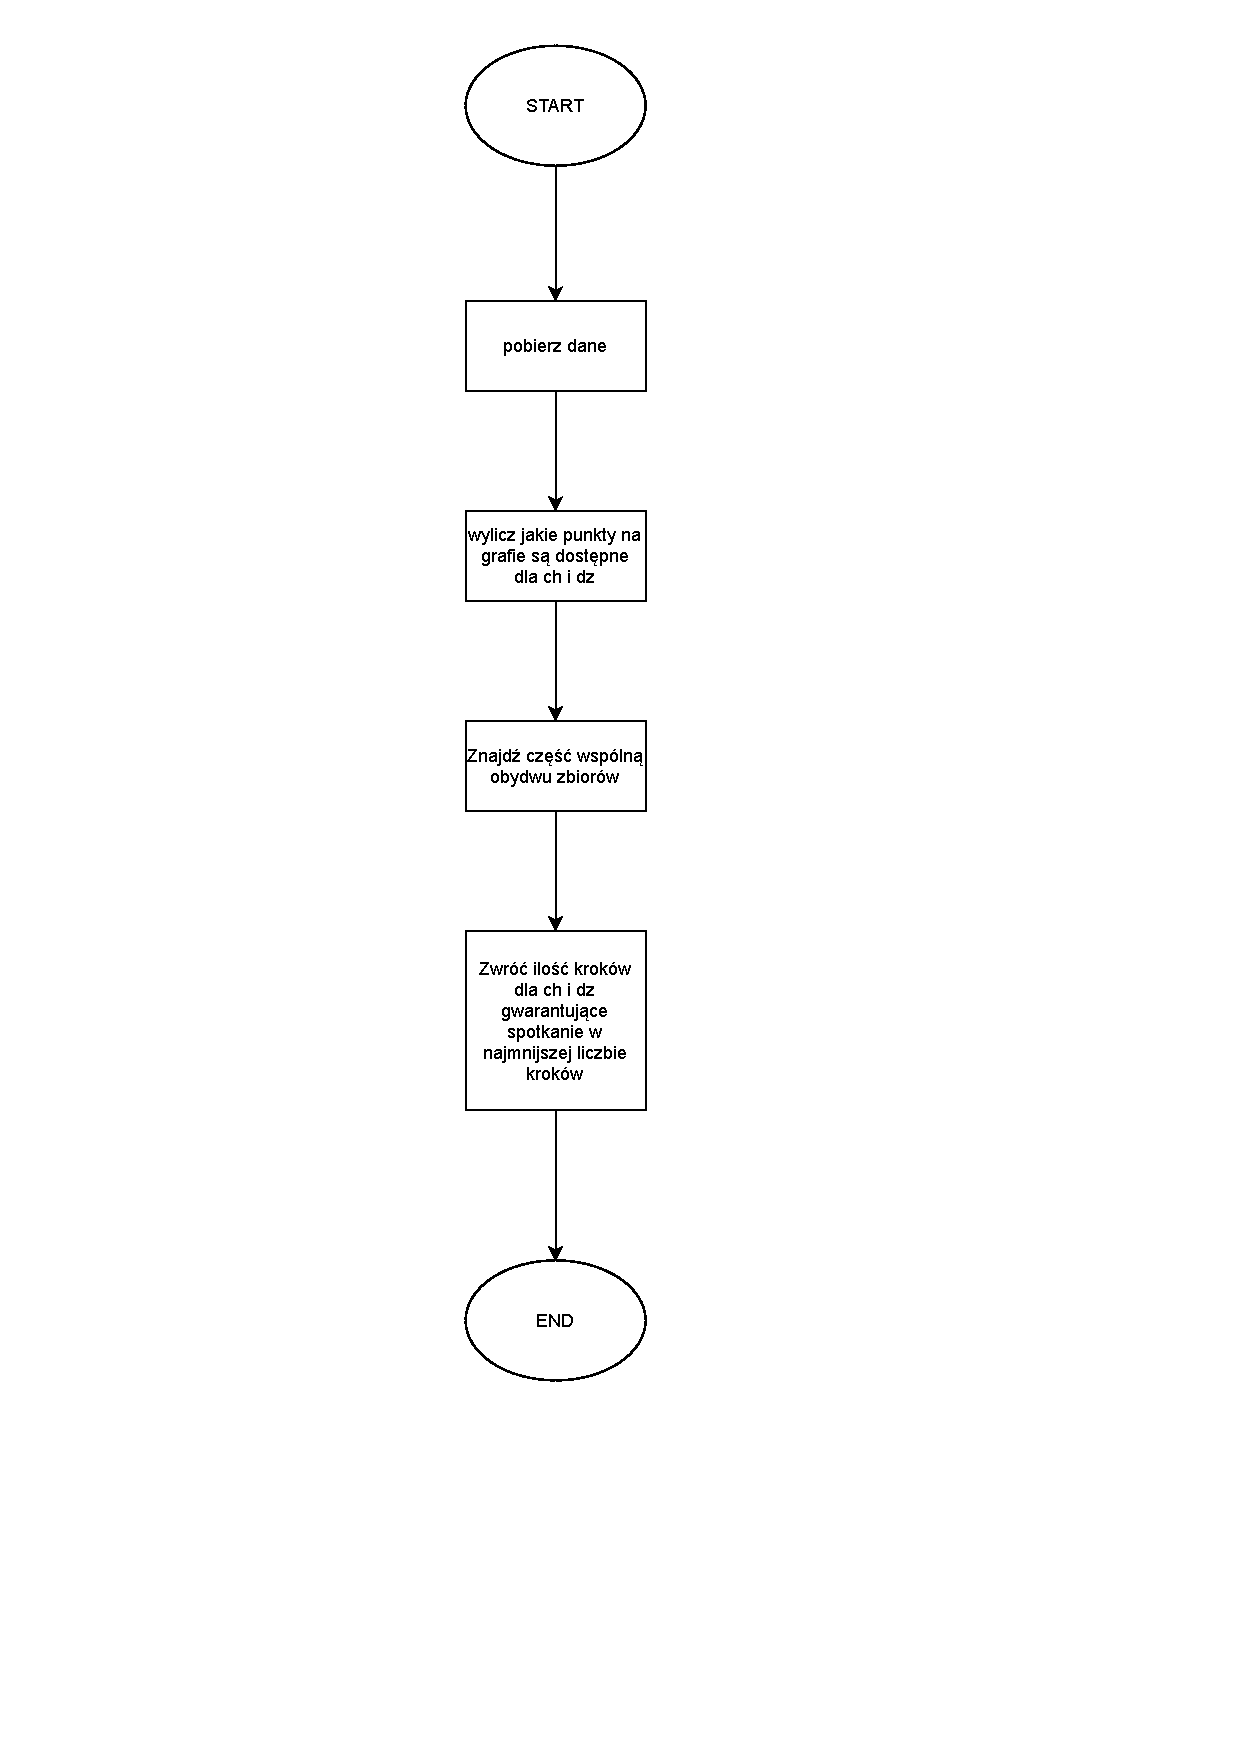
\includegraphics[scale=0.45]{graph.pdf}
	\end{figure}


	\section{Implementacja}
	Opis, zasada i działanie programu ze względu na podział na pliki, nastepnie	funkcje programu wraz ze szczegółowym opisem działania (np.: formie pseudokodu, czy odniesienia do równania) \\
	
	Program menu.bat jest skryptem systemowym, który steruję wszystkimi programami
	
	\begin{tikzpicture}[mindmap, grow cyclic, every node/.style=concept, concept color=orange!40, 
	level 1/.append style={level distance=5cm,sibling angle=90},
	level 2/.append style={level distance=3cm,sibling angle=45},]

    \node{menu.bat}
	child { node {1 Info}}
	child [concept color=green!40]{ node {3 makeHTML.py}
	    child [concept color=blue!30]{ node {Exit code: 0}}
	    child [concept color=blue!30]{ node {Exit code: 1}}
	    }
	child { node {4 Exit}}
	child [concept color=green!40]{ node {2 Solve.py}
	    child [concept color=blue!30]{ node {Exit code: 0}}
	    child [concept color=blue!30]{ node {Exit code: 1}}
	    }
	;
    \end{tikzpicture}
    \\Kod wyjścia 1 - skrypt zadziałał prawidłowo\\
    Kod wyjścia 0 - błąd zapisu danych\\\\
    
    
    \\\\menu.bat
    \begin{lstlisting}
    @echo off
:menu
cls
echo Projekt zaliczeniowy z j�zyk�w skryptowych
echo ==============================
echo 1	Informacja na temat polecenia
echo 2	Wykonaj obliczenia (python)
echo 3	Utworz kopie zapasowa
echo 4	Zako�cz
echo ==============================
set /p select=Wybierz opcje (np. 2):
IF %select%==1 GOTO opt1
IF %select%==2 GOTO opt2
IF %select%==3 goto opt3
IF %select%==4 goto exit
:opt1
echo ====================================================================
echo Polecenie jest nast�puj�ce:
echo Na grafie skierowanym nale�y odnale�� najkrutsz� drog� kt�ra 
echo doprowadzi do spotkania w jednym punkcie 2 agent�w. 
echo 
echo ====================================================================
pause
goto menu
:opt2
echo ====================================================================
python solve.py
If %ERRORLEVEL% == 1 (echo Skrypt zadzia�a� prawid�owo)
If %ERRORLEVEL% == 0 (echo B��d zapisu plik�w wyj�ciowych)
If %ERRORLEVEL% == -1 (echo B��d otwarcia plik�w wej�ciowych)

python makeHTML.py
If %ERRORLEVEL% == 1 (echo Zapis raport w postaci pliku html zadzia�a� prawid�owo)
If %ERRORLEVEL% == 0 (echo B��d zapisu plik�w wyj�ciowych w postaci pliku html)
If %ERRORLEVEL% == -1 (echo B��d otwarcia plik�w wej�ciowych podczas tworzenia raportu)
echo ====================================================================

pause
goto menu
:opt3
echo ====================================================================
echo Kopiowanie folderu %cd%...
echo Usuwanie starej kopii zapasowej...
rmdir /S /Q %userprofile%\Backup
echo Tworzenie nowej kopii zapasowej...
mkdir %userprofile%\Backup
xcopy /e /v "%cd%" "%userprofile%\Backup"
echo ====================================================================
pause
goto menu
:exit
echo Koniec
pause
    \end{lstlisting}
    
    
    
    solve.py
	\begin{lstlisting}]
    import os


## global 

tree_size, flie_count, save_failures,boy_dat, girl_dat = 0, 0, 0, 0, 0

def brute(data):
    # method appends to list every possible path for both boy and girl on a directional 
    # graph and than compares them to find commony aprchablle nodes. It returns numbers 
    # of steeps needed to reach said node for (boy,girl) with shortest path. In case of
    # multiple fitting solutions it returns the one in which girl has to scale the shortest path. 

    tree = data[1]
    for para in range(2, data[0][1]+2):

        #boy
        current_node = data[para][0]-1
        aproachable = dict()
        for i in range(data[0][0]):
            if current_node+1 in aproachable:
                current_node = tree[current_node]-1
                continue
            aproachable[current_node+1]=i
            current_node = tree[current_node]-1

        #girl
        current_node = data[para][1]-1
        aproachable2 = dict()
        for i in range(data[0][0]):
            if current_node+1 in aproachable2:
                current_node = tree[current_node]-1
                continue
            aproachable2[current_node+1]=i
            current_node = tree[current_node]-1

        #common nodes
        combine = {}
        for i in aproachable.keys():
            try:
                combine[(aproachable[i],aproachable2[i])] = (aproachable2[i]**5+aproachable[i]**5)-(aproachable2[i]<aproachable[i]) 
            except KeyError:
                pass # in case keys do not match 
        try:
            return min(combine, key=combine.get)
        except:
            return '(-1,-1)'

### helpres 


def data_miner(f):
    parsed_data=[]
    for line in f.readlines():
        parsed_data.append(line.rstrip().split(" "))
    for i in range(len(parsed_data)):
        for j in range(len(parsed_data[i])):
            parsed_data[i][j] = int(parsed_data[i][j])
    return parsed_data



try:
    for filename in os.listdir(os.path.join(os.path.dirname(__file__), "input")):
        with open(os.path.join(os.path.dirname(__file__),"input", filename), 'r') as f:
                try:
                    
                    file_out = open(os.path.join(os.path.dirname(__file__), "output","output_{}.txt".format(filename)), "w")
                    data = data_miner(f)
                    cst = brute(data)
                    file_out.writelines(str(cst))
                    file_out.close()
                    flie_count+=1
                    girl_dat += cst[1]
                    boy_dat += cst[0]
                    tree_size+=data[0][0]
                except IOError:
                    save_failures+=1
                    file_out = open("failed_files.txt", "a")
                    file_out.writelines("błąd zapisu danych dla danych z przetwarzania pliku {}".format(filename))
                    file_out.close()
except:
    exit(0)
file_out = open("raport.txt", "w")
file_out.writelines("Processed files: \n{}\nFailed files\n{}\nBoy avg:\n{}\nGirl data\n{}\nTree size\n{}".format(flie_count,save_failures,boy_dat, girl_dat,tree_size))
file_out.close()
exit(1)

	\end{lstlisting}
	
	
	
	
	
	\\
	\\makeHTML.py
	\begin{lstlisting}
	# Zapis do pliku html
# Zapis do pliku html
try:
    file_in = open("raport.txt", "r")
    lines = file_in.readlines()
    file_in.close()
except IOError:
    print("Nie znaleziono pliku")
    exit(-1)

try:
    x = int(lines[1])
    y = int(lines[3])
    z = int(lines[5])
    t = int(lines[7])
    q = int(lines[9])
except ValueError:
    print("Nieprawidłowe dane wejściowe, program zostanie wykonany na poniższych danych:")


try:
    file_html = open("output.html", "w")

    message = """
    <!DOCTYPE html>
    <html>
    <head>
    <link rel="stylesheet" href="styles.css">
    </head>
    <body>


    <table class="steelBlueCols">
    <thead>
    </thead>
    <tbody>
    <tr>
    <td>Przetworzone pliki</td><td>"""

    message_res_1 = x
    message_res_4 = y
    message_res_4_1 = q/x
    message_res_3 = "{}|{}".format(z/x,t/x)
    message2 = """
    </td>
    <td>Przetworzone pliki</td><td>"""
    message3 = """
    </td></tr>
    <tr>
    <td>Średnie punkty początkowe(b|g)</td><td>"""
    

    message4 = """
    </td></tr>
    <tr>
    <td>Pliki nieprzetworzone</td><td>"""
    message4_1 = """
    </td></tr>
    <tr>
    <td>Średni rozmiar drzewa</td><td>"""

    
    message5 = """
    </td></tr>
    <tr>
    </tbody>
    </tr>
    </table>

    </body>
    </html>"""
    file_html.writelines(str(message))
    #file_html.writelines(str(message2))
    file_html.writelines(str(message_res_1))
    file_html.writelines(str(message3))
    file_html.writelines(str(message_res_3))
    file_html.writelines(str(message4))
    file_html.writelines(str(message_res_4))
    file_html.writelines(str(message4_1))
    file_html.writelines(str(message_res_4_1))
    file_html.writelines(str(message5))
    file_html.close()
except IOError:
    print("Błąd zapisu danych")
    exit(0)
    
exit(1)
	\end{lstlisting}
	
	

	
	\begin{figure}[!htb]
	    \centering
	    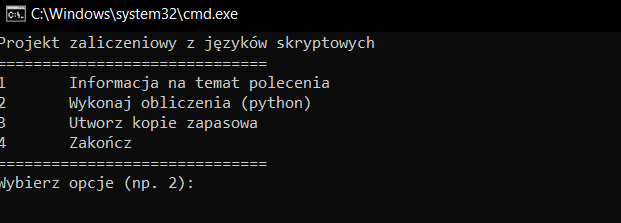
\includegraphics{dzialanie.PNG}
	\end{figure}
		\begin{figure}[!htb]
	    \centering
	    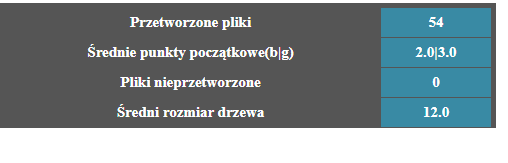
\includegraphics{htl.PNG}
	\end{figure}
	

	
	\newpage
	
    \newpage
	\section{Podsumowanie}
	
	\subsection{Co zostało zrobione}
	\begin{blockquote}
        Program pozwala wczytać wyprowadzone dane, potrzebne do obliczenia czasu, po którym wskazówki zegara ustawią się  jednej linii. Problem matematyczny nie był, aż tak trudny w tym zadaniu co pozwoliło skupić się na integracji skryptów i utrwalenia wiedzy zdobytej w trakcie nauki języków skryptówych.
    \end{blockquote}
    \subsection{Dalsze prace}
	\begin{blockquote}
        Algorytm jest niewydajny, dobrym pomysłem wydaje się tego poprawa.
    \end{blockquote}

    	


\end{document}
